\documentclass[
fontsize=12pt, 	% Taille de police
a4paper, 		% Papier A4
twoside=true, 	% Recto-verso
open=right, 	% Côté d'ouverture
parskip=full,
]{scrreprt}

% Supprime des warnings lors de la compilation avec certains plugins obsolètes.
\usepackage{scrhack}

% Utilisons UTF-8
\usepackage[utf8]{inputenc}
\usepackage[T1]{fontenc}

% Traduire le document en français
\usepackage[french]{babel}

% Pour ajouter des symboles à LaTeX comme ©
% Pourrait probablement être abandonné car non maintenu
% \usepackage{textcomp}

% Pour avoir des liens fonctionnels dans le PDF
\usepackage{hyperref}
\usepackage{url}

% Pour definir et choisir des couleurs
\usepackage[svgnames, table]{xcolor}

% Active la commande \footnote
\usepackage{footnote}

% Permet d'utiliser les guillemets français avec \og et \fg
% https://tex.stackexchange.com/questions/281279/style-of-quotation-marks
\usepackage[autostyle]{csquotes}

% Permet de forcer la présence d'un flotant "ici" avec un grand H
\usepackage{float}

% Permet de placer du texte côte-à-côte avec des figures
% Utiliser avec 
% \begin{wrapfigure}{r}{5cm} FIGURE \end{wrapfigure}
% r/l/i/o désignant le côté et 5cm la taille de la figure (en majuscule plus ou moins)
% CF http://mirrors.standaloneinstaller.com/ctan/macros/latex/contrib/wrapfig/wrapfig-doc.pdf
\usepackage{wrapfig}

% Permet d'utiliser un ensemble de symboles et fonctions mathématiques
\usepackage{amsmath}
\usepackage{amssymb}

% Permet d'ajouter des images
\usepackage{graphicx}

% Permet d'inclure un PDF depuis le code LaTeX, par exemple pour une page de titre customisée (commande includepdf)
\usepackage{pdfpages}

% Permet d'écrire du texte sans sens, ce qui permet une visualisation rapide du thème et des parties pleines
\usepackage{blindtext}

% Calme LaTeX sur la justification à outrance, ce qui évite de couper un mot sur trois
\global\tolerance=2000
\global\hyphenpenalty=30000



% Ce fichier utilise les commandes KOMA-Script pour définir des titres bien plus classes en mode twoside
% Quelques modification ont probablement été faites, mais la plupart vient d'internet

% Permet de choisir le style de page
\usepackage{scrlayer-scrpage}

% Permet de faire tourner les images
\usepackage{rotating}


\definecolor{LightGreen}{RGB}{228, 241, 195}
\definecolor{MediumGreen}{RGB}{201, 228, 134}

\definecolor{LightBlue}{RGB}{191, 215, 237}
\definecolor{MediumBlue}{RGB}{127, 174, 216}
\definecolor{DarkBlue}{RGB}{0, 94, 184}

\definecolor{LightGray}{gray}{.94}
\definecolor{DarkGray}{gray}{.172}


\colorlet{ctcolorchapterline}{LightBlue}
\colorlet{ctcolorchapternum}{MediumBlue}
\colorlet{ctcolorfooterline}{LightBlue}
\colorlet{ctchaptertitles}{DarkBlue}
\colorlet{ctsectiontitles}{DarkBlue}
\colorlet{ctsubsectiontitles}{MediumBlue}



\cfoot*{}
\ofoot*{}

\AddLayersToPageStyle{scrheadings}{pagenumber.odd,pagenumber.even}
\AddLayersToPageStyle{plain.scrheadings}{pagenumber.odd,pagenumber.even}
\DeclareNewLayer[
  foreground,
  oddpage,
  foot,
  contents={%
    \hfill
    \makebox[0pt][l]{%
      \pagenumberrule%
      \hspace*{10pt}%
      \pagemark%
    }%
  }
]{pagenumber.odd}
\DeclareNewLayer[
  clone=pagenumber.odd,
  evenpage,
  contents={%
    \makebox[0pt][r]{%
      \pagemark%
      \hspace*{10pt}%
      \pagenumberrule%
    }%
  }
]{pagenumber.even}
\newcommand*\pagenumberrule{%
  {\color{ctcolorfooterline}\rule[\dimexpr-10cm+\ht\strutbox\relax]{1.25pt}{10cm}}%
}
\addtokomafont{pagenumber}{\usekomafont{disposition}}

\makeatletter
\renewcommand\chapterlinesformat[3]{%
  \ifstr{#1}{chapter}
    {%
      \parbox[b][\ht\strutbox]{\textwidth}{%
        \parbox[b]{\dimexpr\textwidth-3em\relax}{\raggedright#3}%
        \makebox[3em][r]{%
          \hfill
          #2%
        }%
      }%
    }{\@hangfrom{#2}{#3}}% <- original definition for other levels
}
\makeatother
\renewcommand\chapterformat{%
  \textcolor{ctcolorchapterline}{\rule[-5pt]{2pt}{10cm}}%
  \quad
  {\fontsize{60}{60}\selectfont\textcolor{ctcolorchapternum}{\thechapter}}%
}

\renewcommand*\sectionlinesformat[4]{%
  \makebox[0pt][r]{#3}{\textcolor{ctsectiontitles}{#4}}%
}
\setkomafont{chapter}{\normalfont\huge\sffamily\bfseries\color{ctchaptertitles}}
\setkomafont{subsection}{\color{ctsubsectiontitles}}
% Utilisation des glossaires
%
% Dans le préambule, utiliser la commande
% 	\newglossaryentry{latex}
% 	{
% 	    name=latex,
% 	    description={Is a mark up language specially suited 
% 	    for scientific documents}
% 	}
% ou, pour un acronyme,
%  	\newacronym{ALI}{ALI}{Amplificateur Linéaire Intégré}
% 
% A utiliser avec les commandes \Gls{ALI} ou \gls{ALI} dans le texte
%
% Pour afficher le glossaire, les trois lignes suivantes font l'affaire, 
%	\appendix
%	\printglossaries
%	\glsaddallunused % < Pour ajouter les entrées non utilisées dans le texte
%
% Plus d'infos : https://www.overleaf.com/learn/latex/Glossaries

% Importation du package glossaires


\usepackage[
	style=super,
	%nonumberlist,
	toc,
	xindy,
	acronym,
	numberedsection
	]{glossaries-extra}
	
\setabbreviationstyle[acronym]{long-short}
\glssetcategoryattribute{acronym}{glossdesc}{title}
\renewcommand{\glsnamefont}[1]{\textbf{#1}}

\renewcommand*{\glstextformat}[1]{\textsf{#1}}

\makeglossaries

% Ce fichier est à inclure pour activer le support des tableaux

\usepackage{array}
\usepackage{tabularx}
\maketitle
\input{preambule/bibliographie}
% Paquet permettant l'affichage de blocs de code
% Deux moyens de l'utiliser, soit on importe le code depuis un fichier
% 	\lstinputlisting[language={[x86masm]Assembler}, caption=Légende, label=listing:nom_du_label, float]{FICHIER.EXT}
% Soit directement dans le code LaTeX
% 	\begin{lstlisting} et \end{lstlisting}
% Avec les memes options que précédemment.

% On utilise listings pour afficher du code
\usepackage{listings}

%New colors defined below
\definecolor{codegreen}{rgb}{0,0.6,0}
\definecolor{codegray}{rgb}{0.5,0.5,0.5}
\definecolor{codepurple}{rgb}{0.58,0,0.82}
\definecolor{backcolour}{rgb}{0.95,0.95,0.92}


\lstdefinestyle{code_style}{
  backgroundcolor=\color{backcolour},   commentstyle=\color{codegreen},
  keywordstyle=\color{magenta},
  numberstyle=\tiny\color{codegray},
  stringstyle=\color{codepurple},
  basicstyle=\ttfamily\footnotesize,
  breakatwhitespace=false,         
  breaklines=true,                 
  captionpos=b,                    
  keepspaces=true,                 
  numbers=left,                    
  numbersep=5pt,                  
  showspaces=false,                
  showstringspaces=false,
  showtabs=false,                  
  tabsize=2
}

\lstset{style=code_style}
% Ce fichier définit plusieurs boites colorées (definition, proposition, theoreme, remarque, exemple) qui peuvent êtres utilisées de la manière suivante :
% 	\begin{definition}[]{Mot/Expression à Définir}
%		Contenu de la définition
%	\end{definition}
% Et de façon similaire pour les autres types de boites.

% On commence par importer TColorBox
\usepackage[many]{tcolorbox}

% chktex-file 36
% chktex-file 8



% Pour des boîtes de taille variables
\usepackage{varwidth}

\newtcolorbox{definition}[2][]
{enhanced,before skip=2mm,after skip=2mm,colback=black!5,colframe=black!50,boxrule=0.2mm,attach boxed title to top left={xshift=1cm,yshift*=1mm-\tcboxedtitleheight},varwidth boxed title*=-3cm,boxed title style={frame code={\path[fill=tcbcolback!30!black]([yshift=-1mm,xshift=-1mm]frame.north west)arc[start angle=0,end angle=180,radius=1mm]([yshift=-1mm,xshift=1mm]frame.north east)arc[start angle=180,end angle=0,radius=1mm];\path[left color=tcbcolback!60!black,right color=tcbcolback!60!black,middle color=tcbcolback!80!black]([xshift=-2mm]frame.north west) -- ([xshift=2mm]frame.north east)[rounded corners=1mm]-- ([xshift=1mm,yshift=-1mm]frame.north east)-- (frame.south east) -- (frame.south west)-- ([xshift=-1mm,yshift=-1mm]frame.north west)[sharp corners]-- cycle;},interior engine=empty,},fonttitle=\bfseries,title={Définition: #2},#1, colbacktitle=red}

\newtcolorbox{proposition}[2][]
{enhanced,before skip=2mm,after skip=2mm,colback=black!5,colframe=black!50,boxrule=0.2mm,attach boxed title to top left={xshift=1cm,yshift*=1mm-\tcboxedtitleheight},varwidth boxed title*=-3cm,boxed title style={frame code={\path[fill=tcbcolback!30!black]([yshift=-1mm,xshift=-1mm]frame.north west)arc[start angle=0,end angle=180,radius=1mm]([yshift=-1mm,xshift=1mm]frame.north east)arc[start angle=180,end angle=0,radius=1mm];\path[left color=tcbcolback!60!black,right color=tcbcolback!60!black,middle color=tcbcolback!80!black]([xshift=-2mm]frame.north west) -- ([xshift=2mm]frame.north east)[rounded corners=1mm]-- ([xshift=1mm,yshift=-1mm]frame.north east)-- (frame.south east) -- (frame.south west)-- ([xshift=-1mm,yshift=-1mm]frame.north west)[sharp corners]-- cycle;},interior engine=empty,},fonttitle=\bfseries,title={Proposition: #2},#1, colbacktitle=blue}

\newtcolorbox{theoreme}[2][]
{enhanced,before skip=2mm,after skip=2mm,colback=black!5,colframe=black!50,boxrule=0.2mm,attach boxed title to top left={xshift=1cm,yshift*=1mm-\tcboxedtitleheight},varwidth boxed title*=-3cm,boxed title style={frame code={\path[fill=tcbcolback!30!black]([yshift=-1mm,xshift=-1mm]frame.north west)arc[start angle=0,end angle=180,radius=1mm]([yshift=-1mm,xshift=1mm]frame.north east)arc[start angle=180,end angle=0,radius=1mm];\path[left color=tcbcolback!60!black,right color=tcbcolback!60!black,middle color=tcbcolback!80!black]([xshift=-2mm]frame.north west) -- ([xshift=2mm]frame.north east)[rounded corners=1mm]-- ([xshift=1mm,yshift=-1mm]frame.north east)-- (frame.south east) -- (frame.south west)-- ([xshift=-1mm,yshift=-1mm]frame.north west)[sharp corners]-- cycle;},interior engine=empty,},fonttitle=\bfseries,title={Théoreme: #2},#1, colbacktitle=orange}

\newtcolorbox{remarque}[2][]
{enhanced,before skip=2mm,after skip=2mm,colback=black!5,colframe=black!50,boxrule=0.2mm,attach boxed title to top left={xshift=1cm,yshift*=1mm-\tcboxedtitleheight},varwidth boxed title*=-3cm,boxed title style={frame code={\path[fill=tcbcolback!30!black]([yshift=-1mm,xshift=-1mm]frame.north west)arc[start angle=0,end angle=180,radius=1mm]([yshift=-1mm,xshift=1mm]frame.north east)arc[start angle=180,end angle=0,radius=1mm];\path[left color=tcbcolback!60!black,right color=tcbcolback!60!black,middle color=tcbcolback!80!black]([xshift=-2mm]frame.north west) -- ([xshift=2mm]frame.north east)[rounded corners=1mm]-- ([xshift=1mm,yshift=-1mm]frame.north east)-- (frame.south east) -- (frame.south west)-- ([xshift=-1mm,yshift=-1mm]frame.north west)[sharp corners]-- cycle;},interior engine=empty,},fonttitle=\bfseries,title={Remarque: #2},#1, colbacktitle=green}

\newtcolorbox{exemple}[2][]
{enhanced,before skip=2mm,after skip=2mm,colback=black!5,colframe=black!50,boxrule=0.2mm,attach boxed title to top left={xshift=1cm,yshift*=1mm-\tcboxedtitleheight},varwidth boxed title*=-3cm,boxed title style={frame code={\path[fill=tcbcolback!30!black]([yshift=-1mm,xshift=-1mm]frame.north west)arc[start angle=0,end angle=180,radius=1mm]([yshift=-1mm,xshift=1mm]frame.north east)arc[start angle=180,end angle=0,radius=1mm];\path[left color=tcbcolback!60!black,right color=tcbcolback!60!black,middle color=tcbcolback!80!black]([xshift=-2mm]frame.north west) -- ([xshift=2mm]frame.north east)[rounded corners=1mm]-- ([xshift=1mm,yshift=-1mm]frame.north east)-- (frame.south east) -- (frame.south west)-- ([xshift=-1mm,yshift=-1mm]frame.north west)[sharp corners]-- cycle;},interior engine=empty,},fonttitle=\bfseries,title={Example: #2},#1, colbacktitle=gray}


\title{Rapport\\Projet de développement informatique GhostRun}
\author{Arthur JOVART\\Anthony LAMARQUE\\Erwan ALONSO\\Ilyes BENIGHIL}

% Dans le préambule, utiliser la commande
% 	\newglossaryentry{latex}
% 	{
% 	    name=latex,
% 	    description={Is a mark up language specially suited 
% 	    for scientific documents}
% 	}
% ou, pour un acronyme,
%  	\newacronym{ALI}{ALI}{Amplificateur Linéaire Intégré}
% 
% A utiliser avec les commandes \Gls{ALI} ou \gls{ALI} dans le texte

\newglossaryentry{fantome}
{
    name=fantôme,
    description={Un fantôme est un trajet précédent affiché sur la carte. Généralement, notre record personnel.}
}

\newglossaryentry{tag}
{
    name=tag,
    description={Un tag est une étiquette qui permet de catégoriser un trajet.}
}

\newglossaryentry{etat_relax}
{
    name={état "relax"},
    description={Symbolise l'état de l'utilisateur lors de son trajet. Si celui ci est pressé de partir, il n'est pas relax. A l'inverse, si il est en avance, il ne cherchera pas à courir et sera donc considéré comme "relax"}
}


\newacronym{GPS}{GPS}{Global Positioning System}

\begin{document}

% Page de titre
\maketitle




% Sommaire
\tableofcontents

% Chapitre 1: Introduction
\chapter{Introduction}


Ce projet a pour but de permettre à l’utilisateur de connaître le temps mis sur ses trajets et d’optimiser un trajet quotidien.

Pour cela, les trajets sont automatiquement ajoutés dans l’application et il est possible de se mesurer à nos fantômes (traces GPS précédentes) et ainsi de comparer l'efficacité des différents moyens de transports utilisables.

De plus, un ensemble de tableaux de records (par moyen de transport, global, temps d’attente total, vitesse de pointe, par date…) sont disponibles pour comparer, et s’améliorer en rejouant les traces GPS de chaque trajet.

Aussi, lors de l’enregistrement d’un trajet, l’utilisateur peut voir apparaître sur la carte le trajet parcouru par les fantômes de son choix afin de se motiver ou de combattre un précédent record.

Ainsi, l’application ne se limite pas à un seul trajet mais permet l’enregistrement d’une multitude de trajets différents, tous avec leurs records spécifiques.


\chapter{Analyse des besoins (Cahier des charges)}

GhostRun est une \textbf{application Android}, sur laquelle l'utilisateur se connecte pour sauvegarder des traces GPS, appelées trajets, qui s'afficheront sur la carte sous la forme d'un \gls{fantome} pendant ses futurs trajets.

Avant d'enregistrer un trajet, l'utilisateur doit d'abord spécifier son itinéraire (départ et arrivée), et le moyen de transport qu'il utilisera. 

Pendant l'enregistrement, il peut spécifier quelle action il réalise. Par exemple, pour un trajet en train, l'utilisateur passe par les modes "préparation", "marche vers la station", "achat d'un billet", "attente du train", "dans le train", "marche vers la destination".

Lors de l'enregistrement d'un trajet, l'utilisateur voit sur un carte l'ensemble des \glspl{fantome} qu'il a auparavant sélectionné. Il peut ainsi tenter de les dépasser en temps réel. Ces \glspl{fantome} sont représentés par des icônes symbolisant le moyen de transport utilisé par l'utilisateur lorsqu'ils ont été enregistrés. L'application doit être utilisable la nuit, elle intègre donc un mode sombre, dans lequel la carte aborde un terme noir, et ou les icônes des \glspl{fantome} sont moins contrastées.

Après avoir enregistré son trajet, l'utilisateur peut y ajouter des metadonnées : conditions particulières, météo, essoufflement, \gls{etat_relax}. L'application calcule et stocke aussi sa vitesse moyenne, maximale, la distance parcourue et d'autres statistiques.

L'application propose aussi un historique des trajets, sur lequel l'utilisateur peut décider d'afficher le trajet en tant que \gls{fantome} lors de l'enregistrement, consulter les meilleurs trajets (triés sur une multitude de critères tels que ceux énoncés précédemment), consulter ses trajets par moyen de transport (voiture, train, bus, vélo, marche, course, metro, RER, ...)

Un bouton permet à l'utilisateur de partager ses scores et l'ensemble de ses \glspl{fantome} si il le désire.

L'application synchronise en arrière-plan les données générées par les trajets afin de les sauvegarder et de pouvoir les afficher sur un site web annexe.

Ce projet sera considéré comme fini lorsque l’application sera utilisable et lorsque l’utilisateur pourra bien voir les différentes statistiques de ces différentes courses.

\section{Contraintes de délais}

Il existe plusieurs contraintes de délais, il y a tout d'abord trois livrables puis une soutenance en juin.

Le livrable 1 doit être rendu avant le 10 février. Il s'agit de rédiger un pré-rapport avec l'analyse des besoins, une spécification fonctionnelle générale, un regroupement modulaire, ainsi qu'une description du flux des données entre les modules. Ce document évoluera au fur et à mesure que le projet avance.

Le livrable 2 doit être rendu avant le 16 mars. Il s'agit de rendre un prototype du logiciel. Ce prototype sera un squelette des développements futurs du logiciel, toutes les classes utiles à l'application seront définies et toutes les méthodes prévues devront être déclarées et appelées, quitte à ce qu'elles soient vides.

Le livrable 3 doit être rendu avant le 18 mai. Il s'agit de rendre le logiciel, les tests et le rapport. Le rapport doit permettre à une personne qui ne connait rien du projet de pouvoir comprendre celui-ci.

Et finalement, la soutenance aura lieu le 2-3 juin. Il s'agira de présenter le projet à un jury, avec une présentation vidéo-projetée, une démonstration du fonctionnement du logiciel, et la réponse aux questions du jury.

\section{Planification des phases du projet}

L'analyse des besoins et la spécification du projet est réalisée dans le cahier des charges avant le 10 février.

Nous commençons la conception architecturale et la conception détaillée de façon à ce que celle-ci soit terminée avant le 16 mars.

Entre le 16 mars et le 20 avril viendra la phase de codage et de rédaction des tests unitaires.

Entre le 20 avril et le 18 mai nous effectuerons les tests de validation et les modifications avec notre client.

\chapter{Specification Fonctionnelle}

% TODO : A faire
\chapter{Regroupement Modulaire et description des flux de données}

Dans la \autoref{fig:25-regroupement_modulaire}, nous pouvons identifier les multiples parties composant notre application.

\begin{figure}[h]
    \centering
    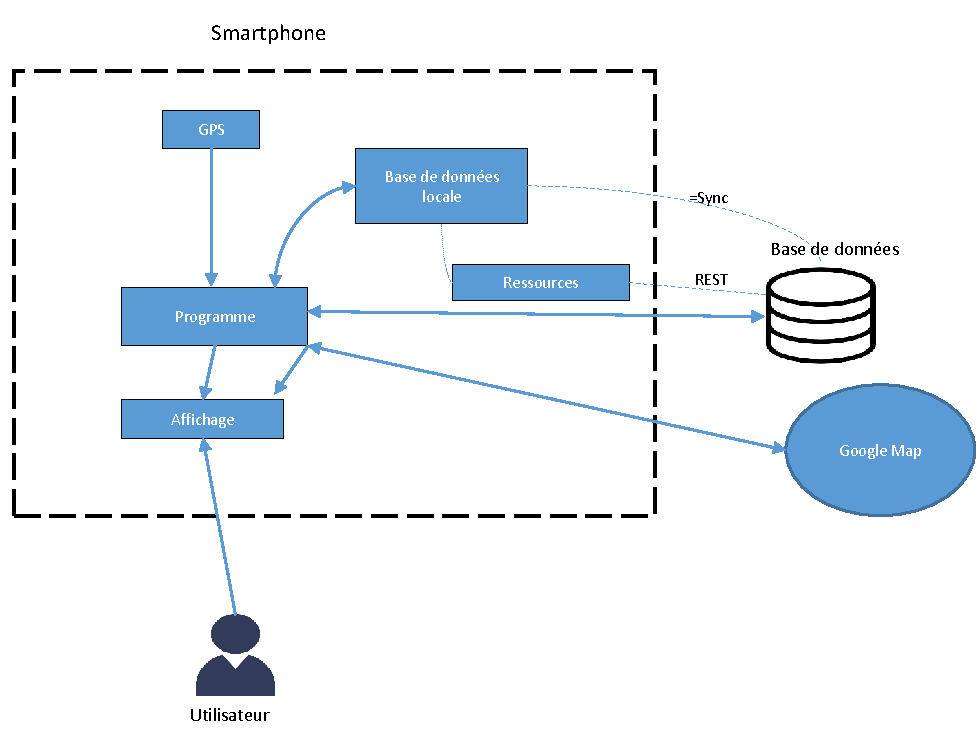
\includegraphics[keepaspectratio, width=2\textwidth/2, height=2\textheight/5]{ima/regroupement_modulaire}
    \caption{Schéma fonctionnel de notre projet.}
    \label{fig:25-regroupement_modulaire}
\end{figure}

\section{GPS}
GhostRun a besoin de récupérer le trajet de l'utilisateur, et pour pouvoir connaitre l'évolution de la position de l'utilisateur
dans le but de l'afficher lors d'un futur trajet. De ce fait l'intervalle de temps entre 2 relevé de position doit être faible.
(de l'ordre de la seconde.)
Le fait de connaitre la position de l'utilisateur à cette fréquence nos permet d'afficher un fantôme qui se déplace de manière continue dans le temps,
mais aussi de connaitre l'évolution de la vitesse au fûr ét à mesure du trajet.
% Expliquer ce que c'est, ce pourquoi l'appli s'en sert et à quelle fréquence, etc..


\section{Base de données}
Nous allons utiliser deux bases de données une locale et une autre à distance. Nous allons stocker différentes informations comme les données et statistiques des différents trajets, les positions favorites des utilisateurs, ces identifiants de connexions et leurs historiques de connexions.
Le programme principal communiquera avec la base de données locale et cette base de données se synchronisera avec la base de données externe. Des ressources devront passer par une \gls{API} \gls{REST} avant d’être stockées sur le serveur distant.


\section{Google Maps}
Nous allons utilisé l'\gls{API} de Google Maps pour avoir la carte sur notre application.
Elle permettra à l'utilisateur de voir sa position actuelle et de préparer une course en choisissant une position de départ et une position d'arrivée.
L'utilisateur pourra de plus enregistrer des positions prédéfinies sur cette carte pour ne pas avoir à réécrire des adresses.
Le programme utilisera cette \gls{API} pour des fonctions comme création d'un trajet ou pour obtenir une position.


\section{Ressources externes}
Les ressources externes permettent de stocker tout ce qui ne peut pas être stocké dans la base de données.
Par exemple, si l'utilisateur souhaite ajouter une image pour décrire son trajet, celle-ci ira dans les ressources externes et à l'aide de l'\gls{API} \gls{REST},
les ressources seront transférés à la base de données externe.


\section{Affichage}
L'interface Homme-Machine permettra à l'utilisateur de voir la carte de Google Maps pour voir sa position actuelle, le trajet en cours,
ainsi que son fantôme en temps réel pour savoir si il arrive à aller plus vite que lui.
Il pourra choisir facilement le trajet de son choix, son moyen de transport et voir ses statistiques sur celui-ci (comme sa vitesse moyenne, maximale).
Tout les trajets enregistrés par l'utilisateur seront consultables à tout moment dans un tableau pour que l'utilisateur voit toutes ses statistiques en appuyant simplement sur un bouton.
Cette interface sera évidemment géré par le programme pour coder ce qui se passera lorsque l'utilisateur appuiera sur tel bouton.
\chapter{Analyse du flux de données}

% TODO : A faire

\chapter{Conclusion}

\appendix
% \chapter{Annexes}

% TODO : C'est à écrire

% Liste des figures
\listoffigures
\glsaddallunused
\printglossaries

% Partie glossaire
%\printglossaries
%\glsaddallunused % < Pour ajouter les entrées non utilisées dans le texte


\chapter{Diagramme de gantt d'avancement du projet}

(Pour une lecture optimale, voir au verso)

\begin{sidewaysfigure}[h]
    \centering
    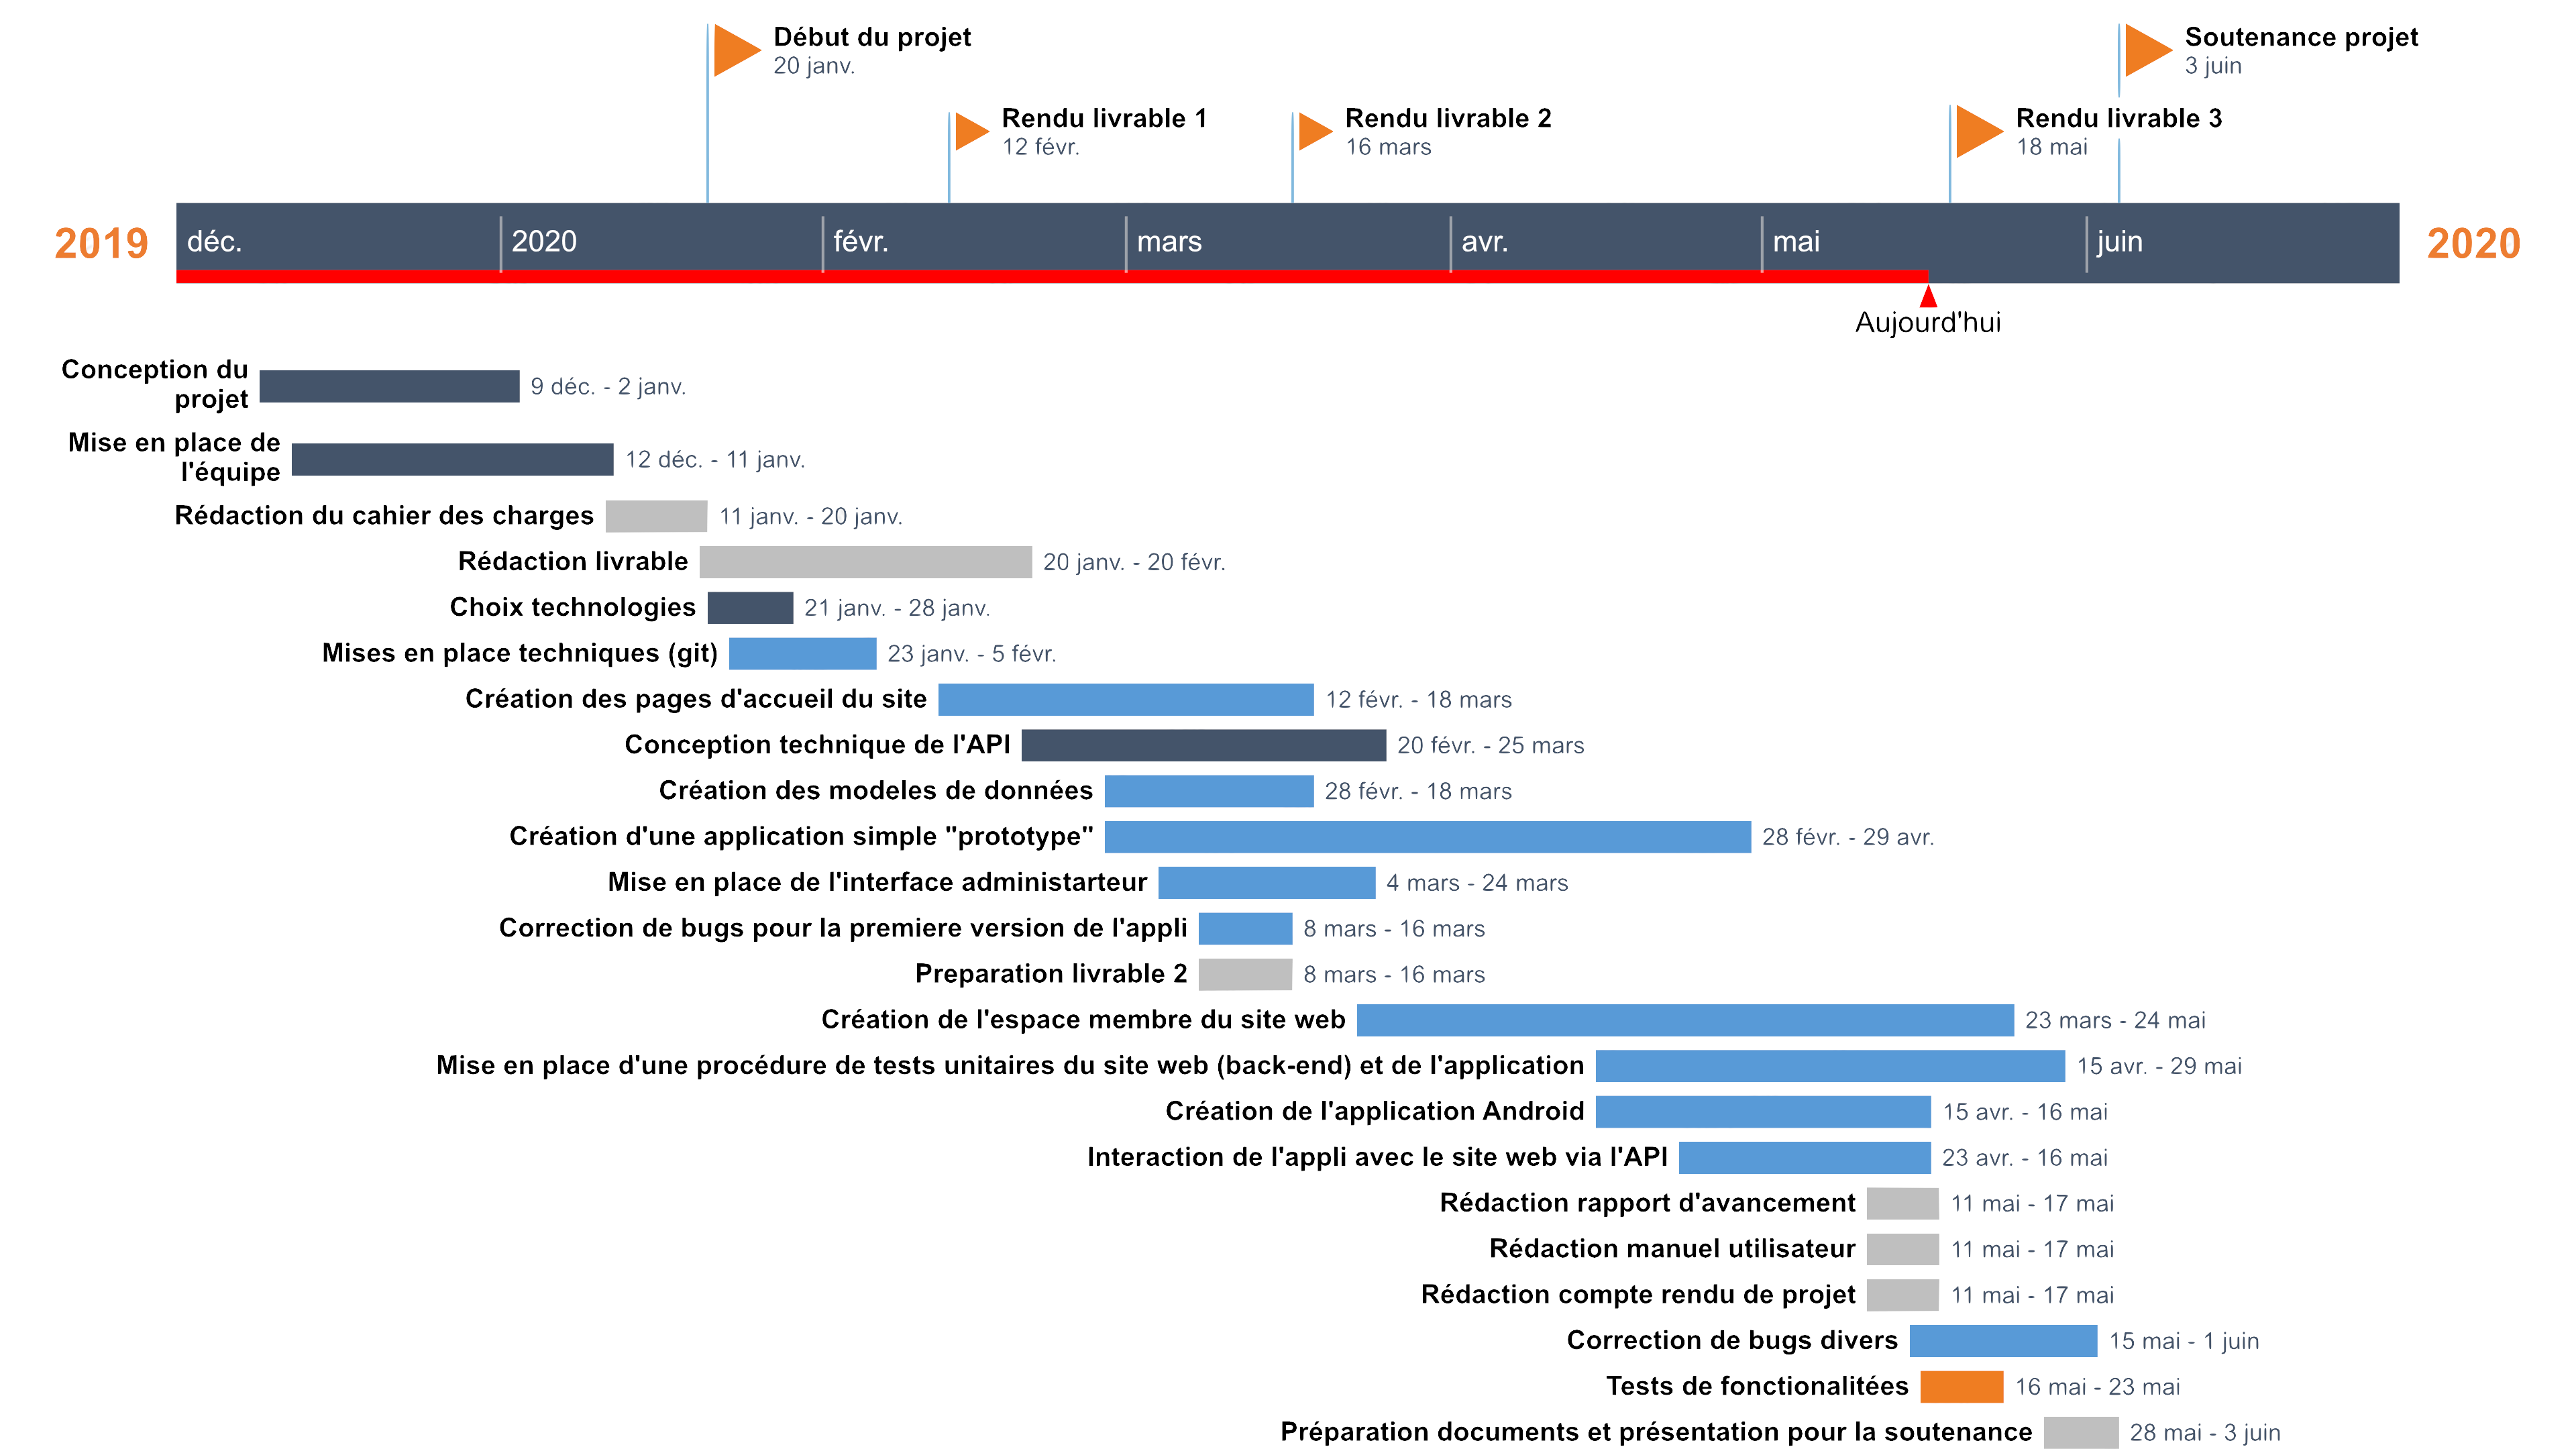
\includegraphics[keepaspectratio, width=\textwidth, height=\textheight]{ima/Planning-gantt}
    \caption{Planning effectif au 16 mai}
    \label{fig:91-Gantt}
\end{sidewaysfigure}


\chapter{Caddyfile pour le deployment du site web en production}

\begin{lstlisting}
(global) {
    # logs
    log {
        output file /var/log/caddy/access.log {
            roll_size 1gb
            roll_keep 5
            roll_keep_for 720h
        }
        format json
    }
    log
    file_server
}

(static_site) {
    import global
}

ghostrun.api-d.com {
    root * /var/www/ghostrun.api-d.com/GhostRun/GhostRunWeb/
    import static_site
    @notStatic {
        not path /static/* /media/*
    }
    reverse_proxy @notStatic localhost:8000
}
\end{lstlisting}





\end{document}
